\section{Set theory and logic}
\label{set-theory}

The theory of sets, typically referred to as \word{set theory}{m{\"a}ngdteori}, forms the basic fundament of all of mathematics. As such, it is probably unsurprising that a huge body of work has been devoted to it. This, however, is not obvious if one simply reads these notes as we will not at all deal with many of the important ideas that underly the theory. Moreover, even though set theory plays an essential role in our study, our treatment of set theory will be rather brief, so the inexperienced reader is also strongly encouraged to study \cite[\S1]{Mun} in detail.

\subsection{Basic notions}
Whereas everything that we will during the course will be as mathematically precise as one can get, we will begin by imprecisely considering a \word{set}{m{\"a}ngd} as a ``collection of things''. These ``things'' will be referred to as the \emph{elements} of the set.

If $A$ is a set, and $a$ is an element of $A$, we write
\[
  a \in A.
\]
Synonymously, we will sometimes say that $a$ is contained in $A$. If on the other hand $a$ is not an element of $A$, then we write
\[
  a \notin A.
\]
If $B$ is another set which contains all the elements of $A$; that is, if $a \in A$ implies that $a \in B$, then we say that $A$ is a \word{subset}{delm{\"a}ngd} of $B$ and write
\[
  A \subset B.
\]
We will also sometimes say that $A$ is contained in $B$ or that $B$ contains $A$. If $A \subset B$ but $A \not= B$, we will write
\[
  A \subsetneq B
\]
and say that $A$ is a \word{proper subset}{{\"a}kta delm{\"a}ngd} of $B$. Set-theoretic relationships are often depicted in so-called Euler diagrams; see Figure~\ref{eulersubset}.
\begin{figure}
  \centering
  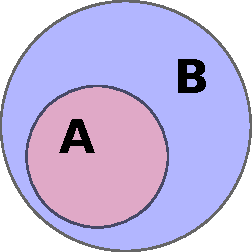
\includegraphics{images/subset.pdf}
  \caption{The Euler diagram representing the inclusion $A \subset B$.}
  \label{eulersubset}
\end{figure}
\begin{example}
  When a set contains only very few elements, one simply lists them. For instance, if $A$ contains only the elements $a$ and $b$, we write $A = \{ a, b\}$. Then if $B = \{ a, b, c\}$, we see for instance that $A \subset B$ and since $c \in B$ but $c \notin A$, we have that $A \not= B$, so $A \subsetneq B$.
  
  Often, sets are given by the properties of their elements, and this will be built into our notation. For instance, the set containing the even numbers will be written
  \[
    \{ x \mid \text{$x$ is an even integer} \},
  \]
  which should be read as ``$x$ such that $x$ is an even integer''.
  
  We will also often be considering the set which contains no elements at all; this set is called \word{the empty set}{den tomma m{\"a}ngden} and is denoted $\emptyset$.
\end{example}
\begin{defn}
  Let $X$ be any set. The \word{power set}{potensm{\"a}ngd} of $X$, denoted $\calP(X)$ is the set of all subsets of $X$, that is
  \[
    \calP(X) = \{U \mid U \subset X \}.
  \]
\end{defn}
\begin{example}
  The elements of power sets are themselves sets which in turn may also have elements. Some examples of power sets are the following:
  \begin{align*}
    \calP(\{a\}) &= \{ \emptyset, \{a \} \}, \\
    \calP(\{a,b\}) &= \{ \emptyset, \{a\}, \{b\} , \{a,b\} \}.
  \end{align*}
  In general, if $X$ is a finite set containing $n$ elements, then $\calP(X)$ contains $2^n$ elements. The only subset of $\emptyset$ is $\emptyset$ itself, which means that
  \[
    \calP(\emptyset) = \{\emptyset\}.
  \]
  Be aware that $\{ \emptyset \}$ consists of a single element, namely $\emptyset$, so it is not itself empty, even though it is tempting to read the notation like that.
\end{example}



\subsection{Cartesian product}

\subsection{Relations}
